%% ****** Start of file apstemplate.tex ****** %
%%
%%
%%   This file is part of the APS files in the REVTeX 4.2 distribution.
%%   Version 4.2a of REVTeX, January, 2015
%%
%%
%%   Copyright (c) 2015 The American Physical Society.
%%
%%   See the REVTeX 4 README file for restrictions and more information.
%%
%
% This is a template for producing manuscripts for use with REVTEX 4.2
% Copy this file to another name and then work on that file.
% That way, you always have this original template file to use.
%
% Group addresses by affiliation; use superscriptaddress for long
% author lists, or if there are many overlapping affiliations.
% For Phys. Rev. appearance, change preprint to twocolumn.
% Choose pra, prb, prc, prd, pre, prl, prstab, prstper, or rmp for journal
%  Add 'draft' option to mark overfull boxes with black boxes
%  Add 'showkeys' option to make keywords appear


\documentclass[reprint,aps,prb,citeautoscript,altaffilletter]{revtex4-2}

%----------------------------------------------------------------------------------------
%
%----------------------------------------------------------------------------------------


%----------------------------------------------------------------------------------------
%	Paquetes
%----------------------------------------------------------------------------------------
%\usepackage[activeacute,spanish,mexico,es-tabla]{babel}
\usepackage[utf8]{inputenc}
\usepackage[T1]{fontenc}
\usepackage{latexsym}
\usepackage{lipsum}
\usepackage{graphics, graphicx}
%----------------------------------------------------------------------------------------
%
%----------------------------------------------------------------------------------------




\begin{document}
	
	
	% -----> TITLE PAGE
	\title{ A development of a Near-Field Optical Microscope }
	\author{\underline{G. A. Mart\'inez-Zepeda}}
	\email{gabmtzz27@gmail.com}
	\author{O. Ruiz-Cigarrillo}
	\email{oscarruiz@cactus.iico.uaslp.mx}
	\author{{K. P. Leija-Alf\'erez}}
	\email{a236792@alumnos.uaslp.mx}
	\author{L. F. Lastras-Mart\'inez}
	\email{lflm@cactus.iico.uaslp.mx}
	\affiliation{Instituto de Investigacion en Comunicaci\'on \'Optica, Universidad Autonoma de San Luis Potos\'i}
	% --->   DATE
	
	\date{\today}
	
	% -----> ABSTRACT	
	\begin{abstract}
		There exist a lot of Scanning Probe Microscopy Systems (SPM), such as Atomic Force Microscopy (AFM) that use a metallic tip and are used to get a image with nanometric resolution, but they are expensive  and in some cases need special conditions for operation, in other hand, the Near-Field Scanning Optical Microscopy (NSOM) systems use a dielectric tip
		and the interaction between the tip and the sample is due optical processes, it makes posible their operation under ambient conditions. In this work we show the first results of the development  of a Near-Field Microscope where its artisanal construction gives it some advantages from comercial ones.
		
	\end{abstract}
	
	\maketitle
    %\include{./files/report-intro.tex}
    %\include{./files/report-results}

	\section{Introduction}
	The optical microscopes are a powerful tools to obtain images of small objects. Their imaging is based on the principle of the
	interference of light waves. Such interference-type microscopes can use not only light waves, but also material waves, such as electron waves, to increase
	the microscopic resolution is limited by diffraction and then we can not measure an object that is smaller than light wavelength \cite{otshu-nf}. To solve this problem appear the
	interaction-based micoscopy that use a probe that interacts with the sample \cite{scannPr}, systems of tis kind of microscopy is the Atomic Force Microscopy (AFM), if the interaction between the tip and the sample is caused by 
	optical fields this is called a scanning near-field optical microscope (NSOM) that the interaction is based in the localization of evanescent waves in the sample\cite{novotny_hecht_2012}, small apertures at the apex of tapered optical fibers are the most widely used
	optical near-field probes. The fiber has to be covered by a metal coating to confine the light and to prevent light leaking out of the tapered end \cite{otshu-nf, scannPr}.
	\par There are different configurations for SNOM using optical fiber tips. The sample can be illuminated from the rear side in a geometry where total internal reflection is found. The lateral variation of the evanescent field in front of the surface is probed
	by detecting the light which couples into the fiber while scanning in close proximity \cite{otshu-nf2}. The intensity of the detected light decays exponentially with the tip–sample distance
	and this mode has therefore been called scanning tunneling optical microscopy. The more widely used configuration is coupling of light into the fiber and illumination of the sample by the near field emerging from the nano-aperture at the fiber apex. The
	resulting light radiation can be detected by far-field detectors \cite{scannPr}.

	\par The distance control in SNOM is more difficult than in other SPM methods due to the fact that the light intensity versus distance curve is very complicated and often non-monotonic \cite{otshu-nf2}. Therefore, it cannot be used for the distance control. Instead, the damping of a lateral oscillation
	of the fiber due to shear forces between apex and sample is exploited. The fiber is excited into oscillation by means of a small quartz tuning fork attached to it, and the change in resonance parameters of the oscillation (usually the phase between excitation and oscillation) is used for the distance feedback controller \cite{otshu-nf}.
	\par The applications of SNOM are numerous for example the ability of SNOM to study the optical activity of single molecules is of great importance for studies of biologically functional systems, Technological applications include the analysis of optical waveguides \cite{paper1}. The electronic structure
	of semiconductor nanostructures has been studied with femtosecond time-resolved SNOM \cite{doi:10.1063/1.126446} and a scientific application is the measurement of the propagation of plas-
	mons excited in structured metal films \cite{PhysRevB.63.155404}.

	\par In section \ref{sys} we explain the experimental setup used in this work, section \ref{samp} gives some information about the sample used to characterize the system, section \ref{res} shows the results obtained in this work and finally we show our conclusions in section \ref{conc}.

	\section{System} \label{sys}
	\begin{figure}[!hbt]
		\centering
		\includegraphics[scale=0.35]{figures/systemNSOM.pdf}

		\caption{NSOM setup developed in this work.}
		\label{fig:Sys}
	\end{figure}

	The system is shown in figure \ref{fig:Sys}, is a collection mode SNOM that means  the use a optical fiber tip to collect the laser light (indicated as Laser1 in the figure \ref{fig:Sys}) that incides in the sample from the far field.The micropositioning system (Micro and nano position) consist of three Newmark linear satges  with micrometric resolution used to control te position of the sample in three dimension, one stage is implemented to to bring the sample closer to the tip (dir $z$) and the other two are used for  scanning the sample (dir $x$ and $y$).
	To scan the sample with nanometric resolulion a PI nanometric stage is placed over the dir $z$ linear stage, the sample is placed on a sample holder over this nanometric stage. To see the sample sposition we use a monochromatic CCD Camera pixeLink with a telecentric lenses and a microscope objetive, to see the sample and the tip an external illumination is needed, the figure \ref{fig:ts} shows the tip and the sample used in the present work. 
	\begin{figure}[!hbt]
		\centering
		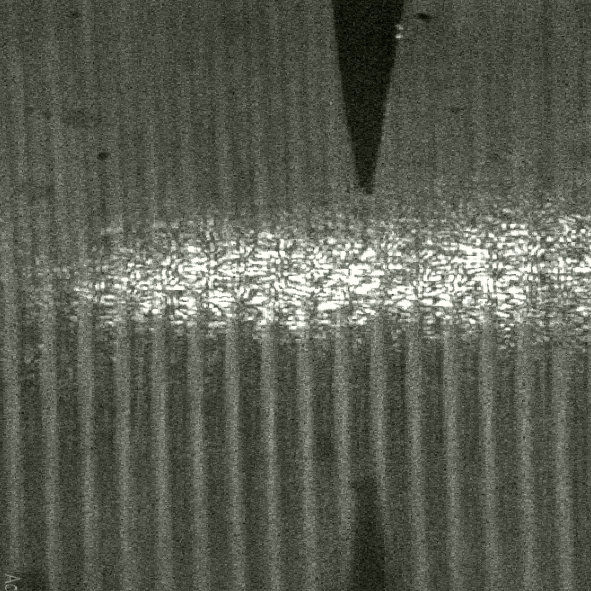
\includegraphics[scale=0.5]{figures/tipSample.pdf}

		\caption{Image of a Sample and the tip using a CCD camera.}
		\label{fig:ts}
	\end{figure}

	\par The sample-tip distance is controlled by the vibration of the tip caused by a piezoelectric attached to the probe, this vibration is monitored  using a second laser incident on the tip of the fiber making possible to see the amplitude and the frequency using the diffraction pattern, because of the near field ineractions the amplitude and  the vibrational frequency have small changes (the frequency changes $0.05 ~Hz$) and when the probe and the sample are in the near-field region
	 a phototube detects the light collected by the probe, because the light intensity is very small we use a lock-in  amplifier to adquire the signal.
	To control all the system was developed a software in LabVIEW, this program has two section, the first one allows the user see and maniplate the position of the sample, and the second is used to make NSOM measurements.

	\section{Sample} \label{samp}

	The sample used in this work to test our instrument is a InP diffraction rating with a period $\Lambda$ of $50~\mu m$ and a duty cycle of $50 \% $, the sample was fabricated using plasma enhanced-chemical vapor deposition (PECVD), photolitography methods and dry etching \cite{Panah:16} .

	\section{Results} \label{res}

	In the figure \ref{fig:afmEx} we show the topographic image of InP grating, this figure was obtained using the Newmark's linear stages, 
	this image shows that the instrument has the capability of measure a micrometer sized object in contrast with comercial ones, in other hand
	we can se that the dimension of the granting is not the same for every period, this problem is caused by the accuracy of the linear stages because they
	are designed to operate in steps larger than $50~\mu m$.
	
	\begin{figure}[!hbt]
		\centering
		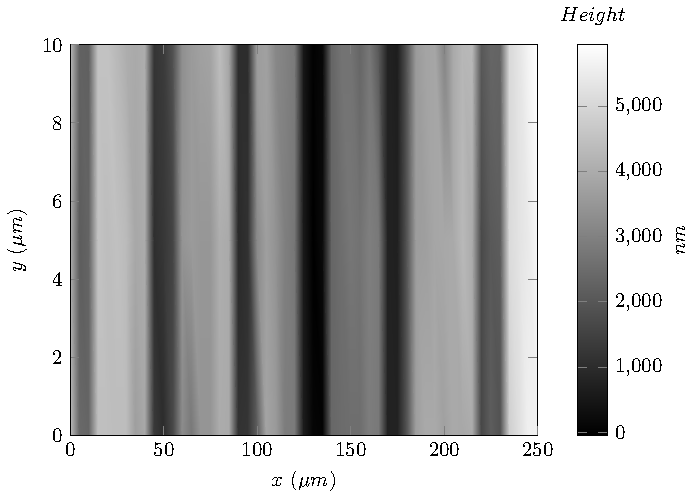
\includegraphics[scale=0.6]{figures/result/extafmImag/exAFMImag.pdf}

		\caption{Topographic image of InP Grating in a region of $250 \times 10 ~ \mu m$.}
		\label{fig:afmEx}
	\end{figure}

	The next step is the measurement of near-field image, we use the nanometric positioner to scan the sample in steps of $2~ \mu m$, the figure \ref{fig:afmim2} shows the topographic image and give information about the shape of the
	measurement region, we can see that the height is about $2.5~\mu m$ and the its period is $25~\mu m$ in accordance with published data. The figure \ref{fig:afmsom} shows the intensity detected by phototube, we can note that the period is the same of the topographic image, 
	and we can observe a contrast between the top and bottom  regions, this is casued by the rugosity and the dopand of InP in these regions.

	\begin{figure}[!hbt]
		\centering
		\includegraphics[scale=0.6]{figures/result/afmImag/AFMImag.pdf}

		\caption{Topographic image of InP Grating measured in a region of $88 \times 10 ~ \mu m$.}
		\label{fig:afmim2}
	\end{figure}

	\begin{figure}[!hbt]
		\centering
		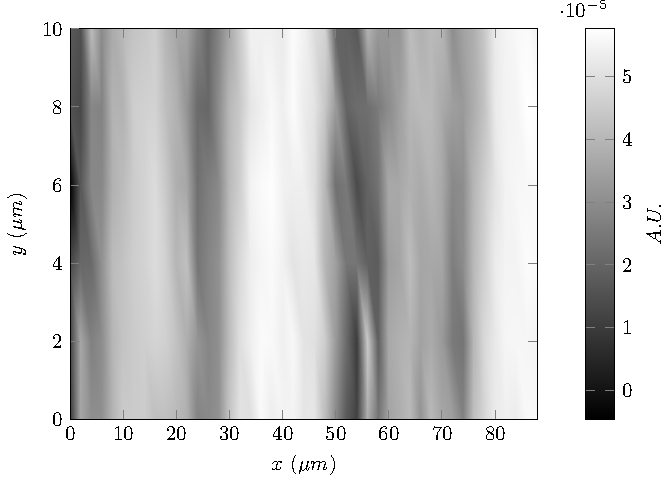
\includegraphics[scale=0.6]{figures/result/nsomImag/nsomImag.pdf}

		\caption{NSOM image of InP Grating measured in a region of $88 \times 10 ~ \mu m$.}
		\label{fig:afmsom}
	\end{figure}

	The figure \ref{fig:comp} shows the comparison between the topographic and nsom profile,  the reduction of dectected signal at the grating edges  is noticeable. we can say that this effect is a topographic artifac because we analized de amplitude change of the vibration of the tip and we can see that the variation is smaller 
	at the edges than in the other regions of the sample that means that the distance between the sample and the tip si larger than the other region and it causes the reduction of signal, in contrast the changes in other regions the changes of the amplitude essentially are the same and this is the reason that we can say that our instrument can obtain 
	optical properties that changes locally.
	
	\begin{figure}[!hbt]
		\centering
		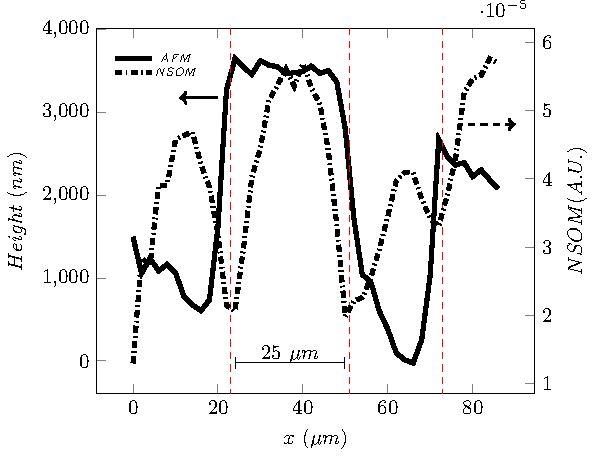
\includegraphics[scale=0.65]{figures/result/compProf/compafmnsom.pdf}

		\caption{comparison bewteen profiles of topographical and NSOM measurements.}
		\label{fig:comp}
	\end{figure}

	\section{Conclusions} \label{conc}
	An automation software capable of performing simultaneous topographic and near field measurements was developed usign LabVIEW, The artisanal construction of the instrument allows 
	some characteristics that are more difficult to implement in comercial ones such as the micrometer sized obejct measurement, spectroscopic measurements at the nanoscale and the control of polarization using 
	a photoelastic modulator. In this work we showed the first measurements used to test the system  and we could obtain a topographic image with microscopic resolution that is similar with optical ones, the signal obtained by the phototube.
	gives information about grating's local optical properties. 

	\bibliographystyle{plain}
	\bibliography{biblio}
	%\nocite{*}
	
\end{document}

